\documentclass{beamer}
\usepackage{relsize}
\usepackage{color}
\usepackage{rotating}

\usepackage{listings}
\usetheme{CambridgeUS}
%\usepackage{beamerthemesplit} % new 
\usepackage{enumitem}
\usepackage{amsmath}                    % See geometry.pdf to learn the layout options.\includeonlyframes{current}
\usepackage{amsthm}                   % See geometry.pdf to learn the layout options. There 
\usepackage{amssymb}                    % See geometry.pdf to learn the layout options. 
\usepackage[utf8]{inputenc} 
\usepackage{graphicx}
\usepackage[english,bulgarian]{babel}
\usepackage{changepage} 

\lstset{language=C++,
                basicstyle=\ttfamily,
                keywordstyle=\color{blue}\ttfamily,
                stringstyle=\color{red}\ttfamily,
                commentstyle=\color{green}\ttfamily,
                morecomment=[l][\color{magenta}]{\#}
}

\setbeamertemplate{itemize items}[circle]

\newtheorem{mydef}{Дефиниция}[section]
\newtheorem{lem}{Лема}[section]
\newtheorem{thm}{Твърдение}[section]
\newtheorem*{remark}{}

\DeclareMathOperator{\restrict}{\upharpoonright}

\setitemize{label=\usebeamerfont*{itemize item}%
  \usebeamercolor[fg]{itemize item}
  \usebeamertemplate{itemize item}}

\setbeamercovered{transparent}



\begin{document}
\title[Увод в програмирането]{Работа с двоични файлове} 
\author{Калин Георгиев}
\frame{\titlepage} 


\section {Двоични файлове}

\begin{frame}
\centerline{Двоични файлове}
\end{frame}


\begin{frame}
\centerline{Двоични файлове}
\vspace{75px}
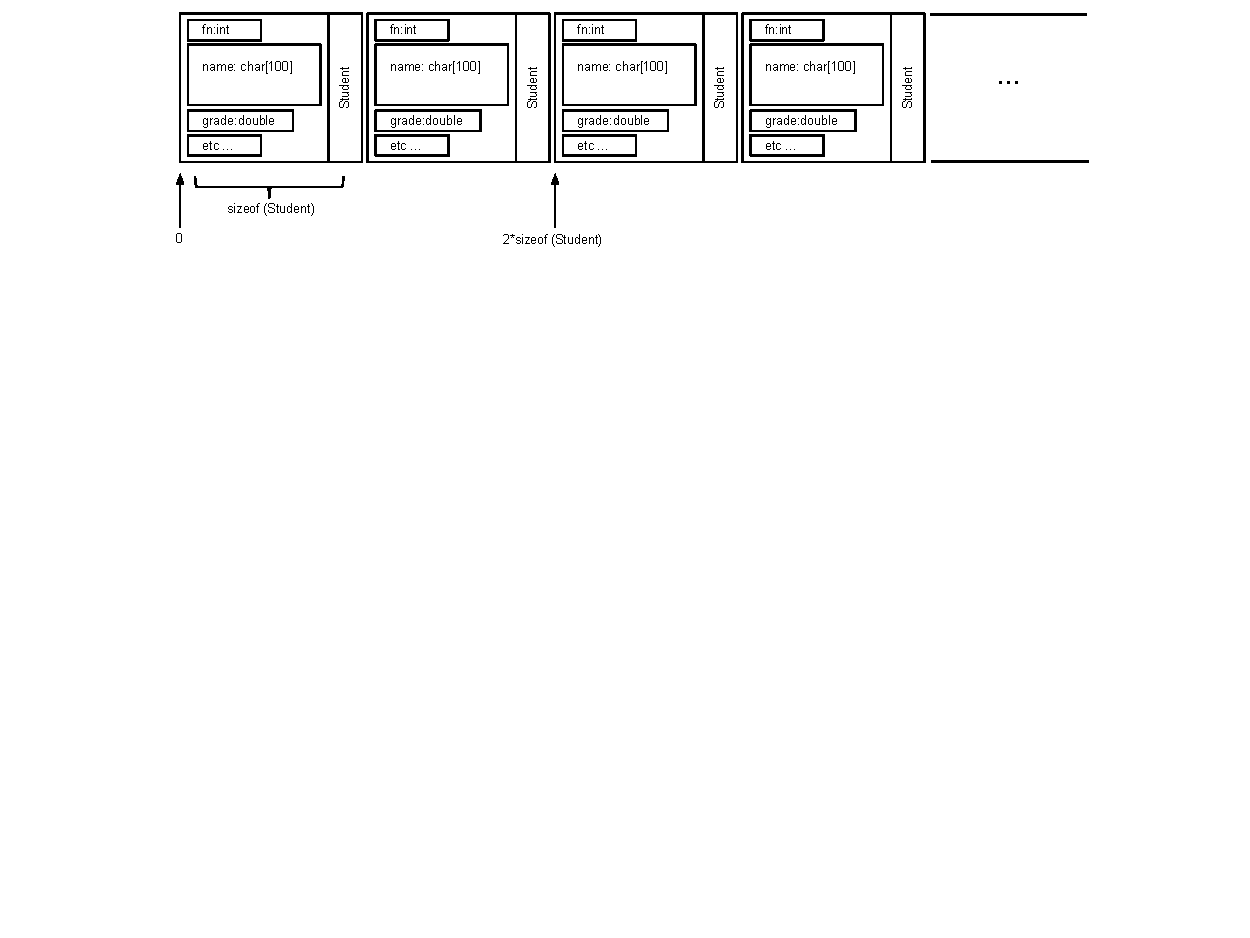
\includegraphics[width=12cm]{images/binfile}
\end{frame}



\begin{frame}[fragile]
\frametitle{Писане в двоичен файл}



\begin{columns}[t]
  \begin{column}{0.6\textwidth}
      %\vspace{-150px}
      \begin{flushleft}
      \relscale{0.65}
      \begin{lstlisting}
//TEXT FILE
ofstream out_file ("myfile.txt");
for (int i = 0; i < 3; i++)
{
  out_file << students[i].fn 
           << " "
           << students[i].name 
           << endl 
           << students[i].grade 
           << endl;
      \end{lstlisting}
\begin{lstlisting}
//BINARY FILE
  ofstream out ("stundets.bin",ios::binary | ios::app);
  for (int i = 0; i < 3; i++)
    out.write ((char*)&students[i],sizeof (Student));

      \end{lstlisting}
\begin{remark}[]
    \texttt{write (char *buffer, size\_t bytes)}
\end{remark}      
      \end{flushleft} 
  \end{column}
  \begin{column}{0.4\textwidth}

  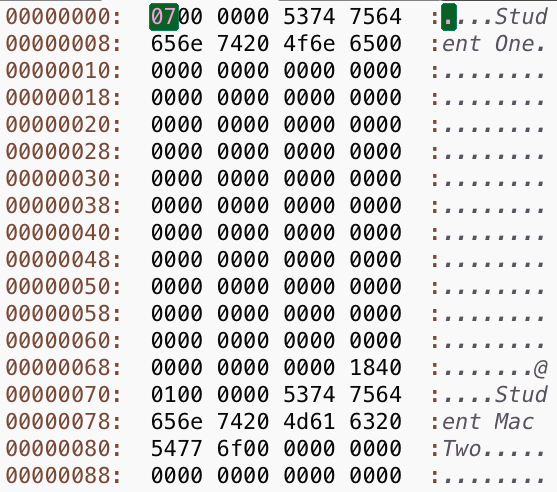
\includegraphics[width=4.5cm]{images/binfiless}
  \end{column}
\end{columns}
\end{frame}


\begin{frame}[fragile]
\frametitle{Четене от двоичен файл}



\begin{columns}[t]
  \begin{column}{0.6\textwidth}
      %\vspace{-150px}
      \begin{flushleft}
      \relscale{0.65}
      \begin{lstlisting}
//OUTPUT
  ofstream out ("stundets.bin",
                ios::binary | ios::app);
  for (int i = 0; i < 3; i++)
    out.write ((char*)&students[i],
               sizeof (Student));
\end{lstlisting}
\begin{lstlisting}  
//INPUT
  ifstream in ("stundets.bin",
               ios::binary);
  Student s;
  while (in.read ((char*)&s, sizeof (Student)))
  { printStudent (s); }
      \end{lstlisting}
\begin{remark}[]
    \texttt{read (char *buffer, size\_t bytes)}

    \texttt{write (char *buffer, size\_t bytes)}
\end{remark}      
      \end{flushleft} 
  \end{column}
  \begin{column}{0.4\textwidth}

  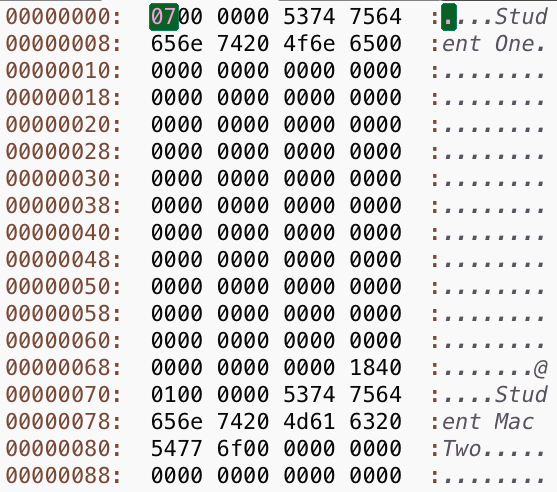
\includegraphics[width=4.5cm]{images/binfiless}
  \end{column}
\end{columns}
\end{frame}


\begin{frame}[fragile]
\frametitle{Двоичен файл / RAM}



\begin{flushright}
\relscale{0.65}
  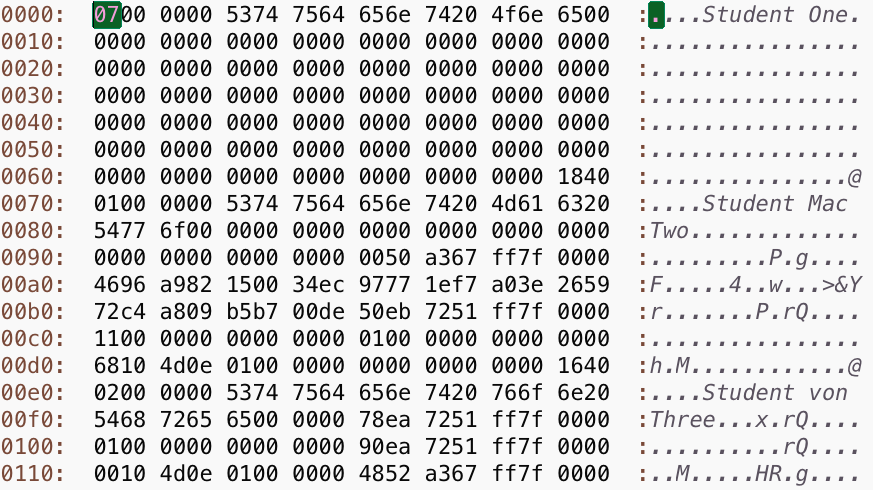
\includegraphics[width=6.5cm]{images/binfilesslarger}
\end{flushright}

\vspace{20px}
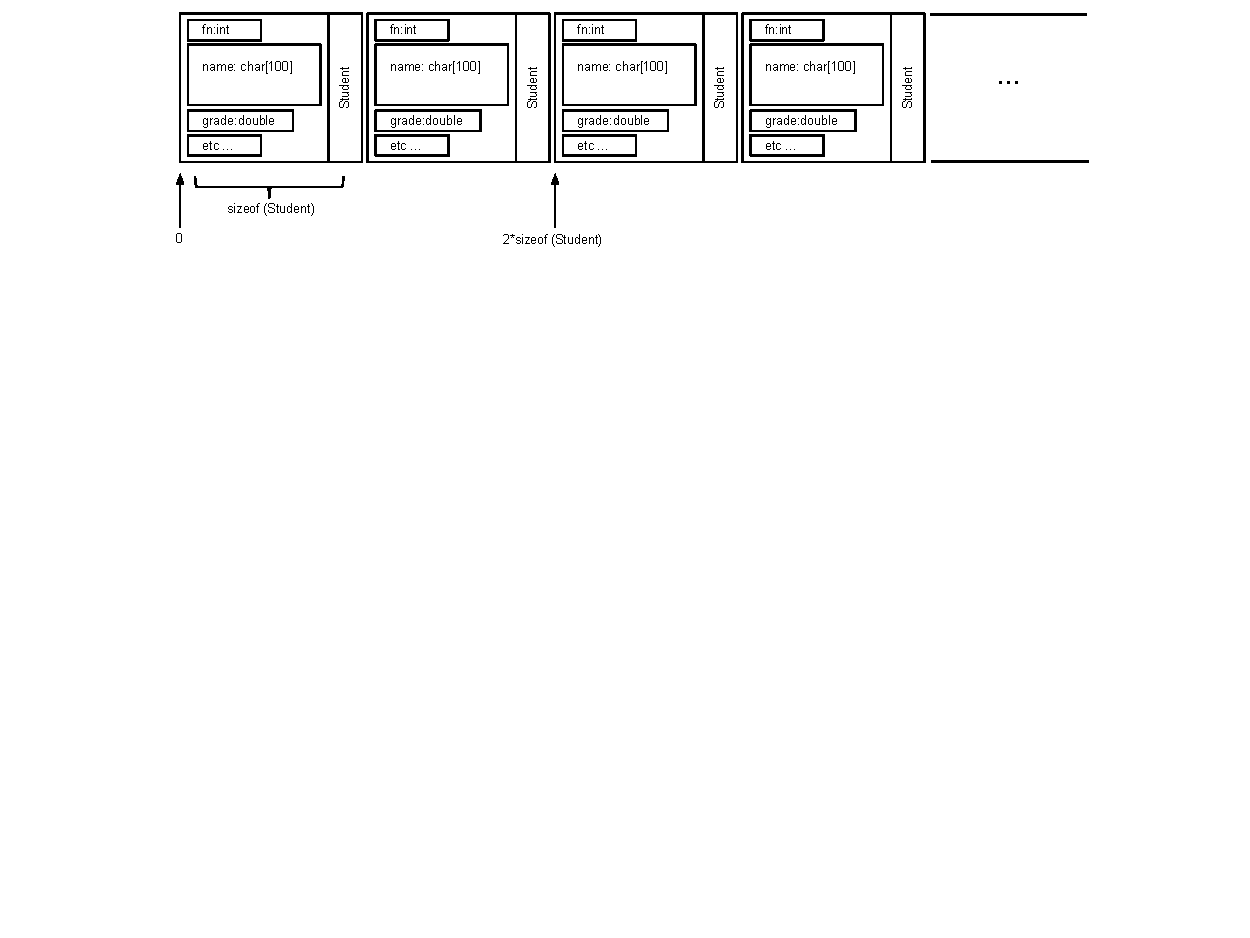
\includegraphics[width=12cm]{images/binfile}


\end{frame}




\begin{frame}[fragile]
\frametitle{Двоичен файл vs. Текстов файл}



\begin{flushright}
\relscale{0.65}
  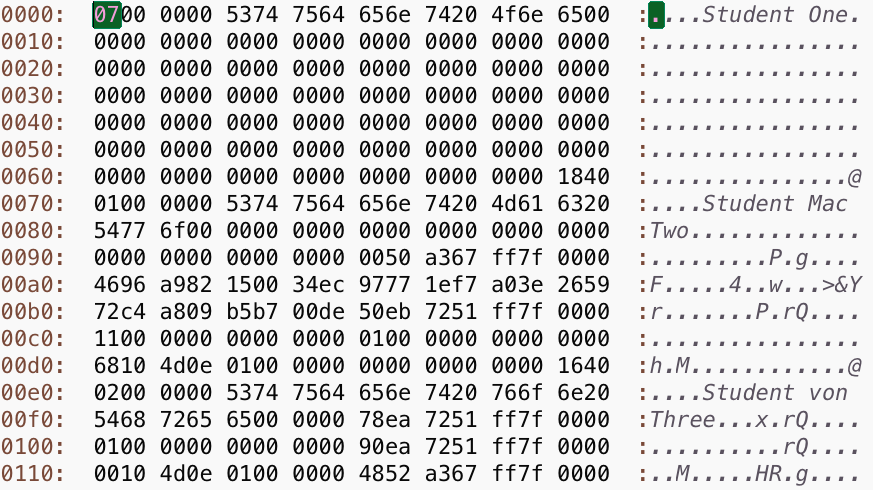
\includegraphics[width=6.5cm]{images/binfilesslarger}
\end{flushright}

\vspace{20px}
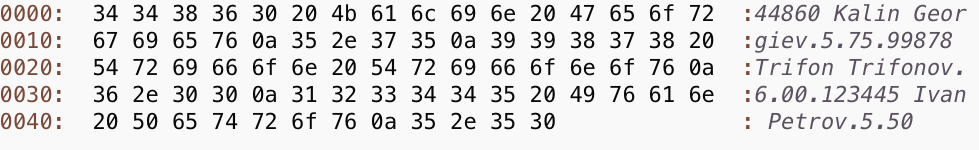
\includegraphics[width=12cm]{images/textfilebin}


\end{frame}



\begin{frame}[fragile]
\frametitle{Позициониране}

\vspace{-20px}



\begin{columns}[t]
  \begin{column}{0.5\textwidth}

\begin{flushleft}
\relscale{0.65}
\begin{lstlisting}
Student s;
//INPUT
ifstream in ("stundets.bin",
             ios::binary);
in.seekg(2*sizeof(Student));
in.read ((char*)&s, sizeof (Student));
printStudent (s);

//OUTPUT
ofstream out ("stundets.bin",
              ios::binary | ios::app);
out.seekp(2*sizeof(Student));
out.write ((char*)&s,sizeof (Student));

\end{lstlisting}
\end{flushleft}   


  \end{column}
  \begin{column}{0.5\textwidth}
\begin{flushright}
\relscale{0.65}
  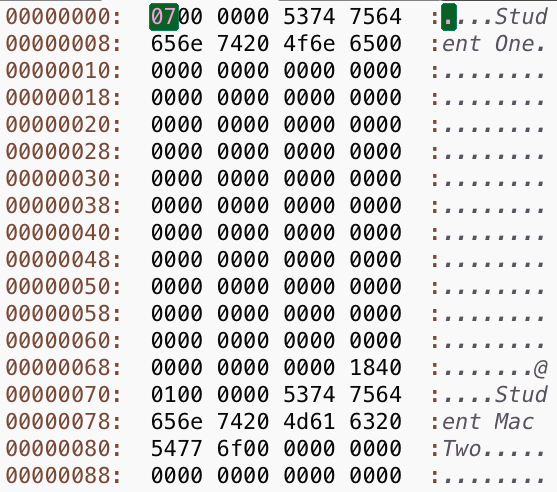
\includegraphics[width=4.5cm]{images/binfiless}
\end{flushright}

  \end{column}
\end{columns}



%\vspace{-10px}
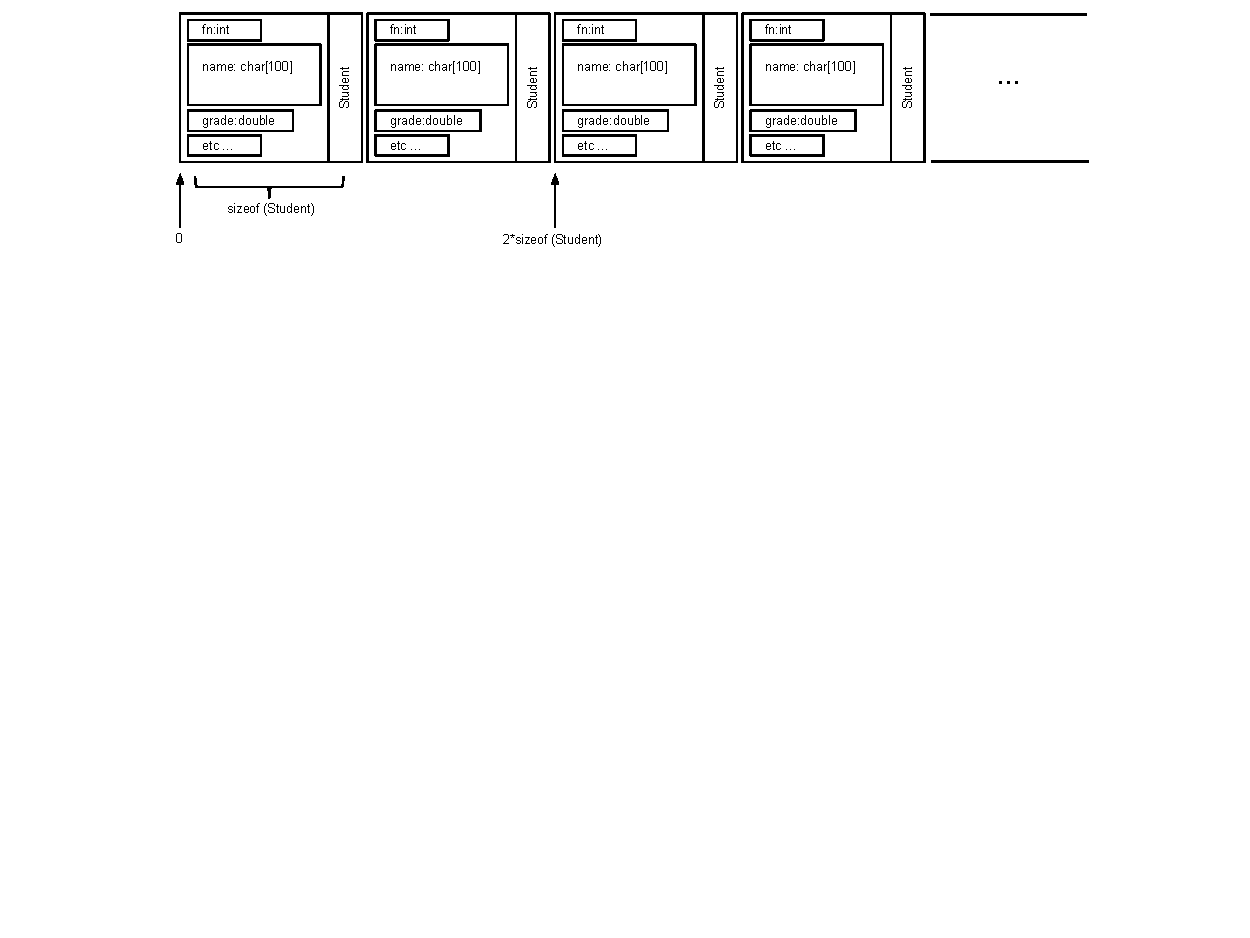
\includegraphics[width=12cm]{images/binfile}


\end{frame}


\begin{frame}[fragile]
\frametitle{Изтриване от двоичен файл}

\begin{flushright}
\relscale{0.65}
  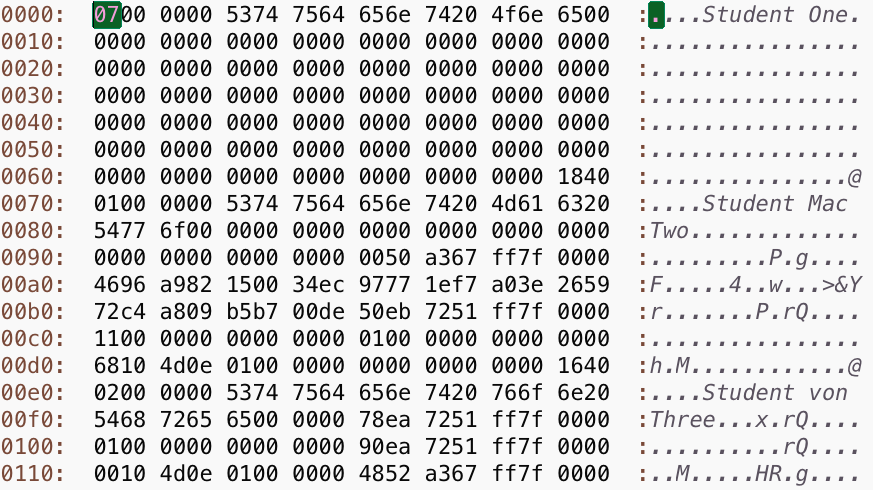
\includegraphics[width=6.5cm]{images/binfilesslarger}
\end{flushright}

\vspace{20px}
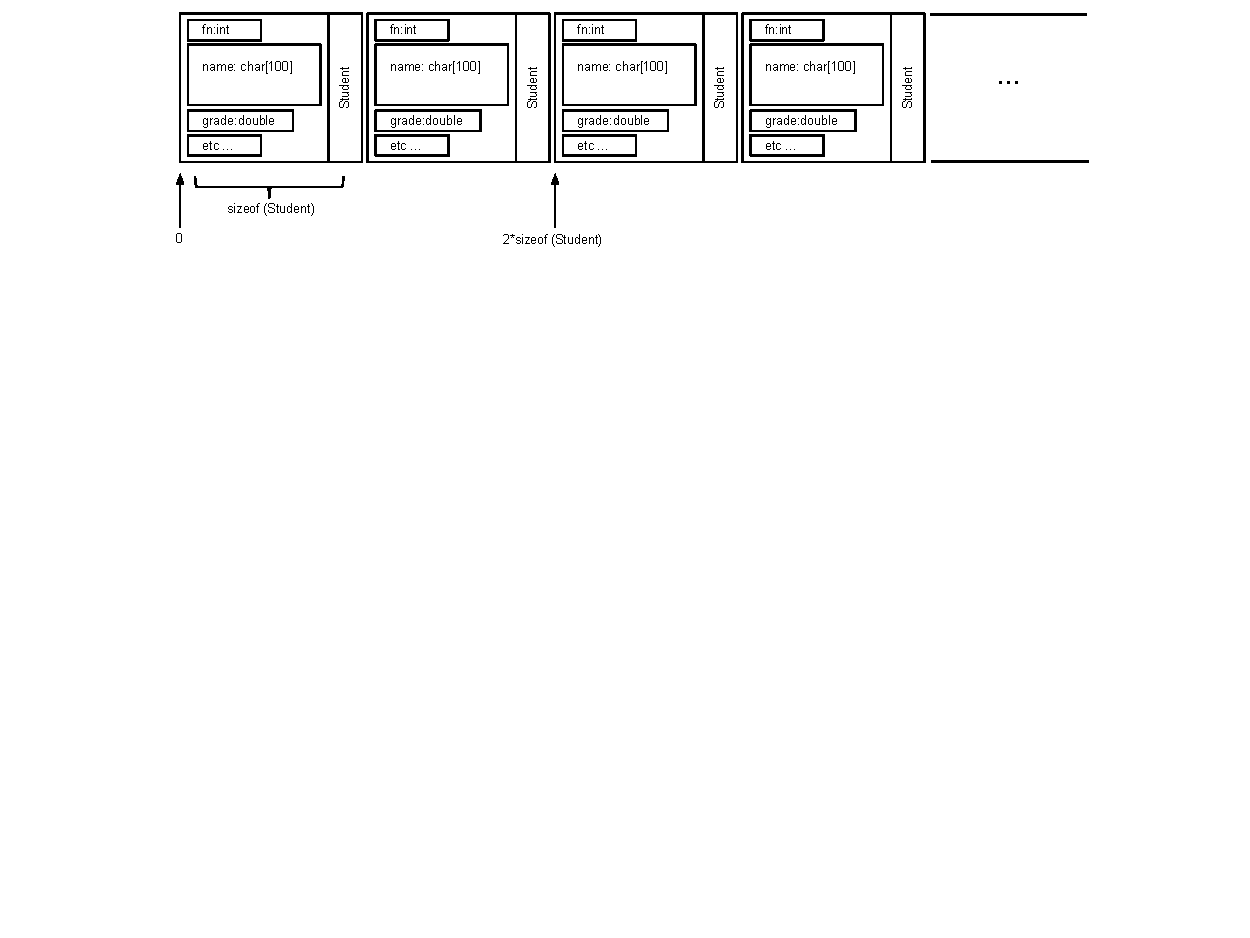
\includegraphics[width=12cm]{images/binfile}


\end{frame}


\begin{frame}[fragile]
\frametitle{struct Student}


\begin{columns}[t]
  \begin{column}{0.5\textwidth}
      \vspace{-350px}
      \begin{flushleft}
      \relscale{0.85}
      \begin{lstlisting}
      struct Student
      {
        bool deleted;
        int fn;
        char name[100];
        double grade;
      };
      \end{lstlisting}
      \end{flushleft} 
  \end{column}
  \begin{column}{0.5\textwidth}
  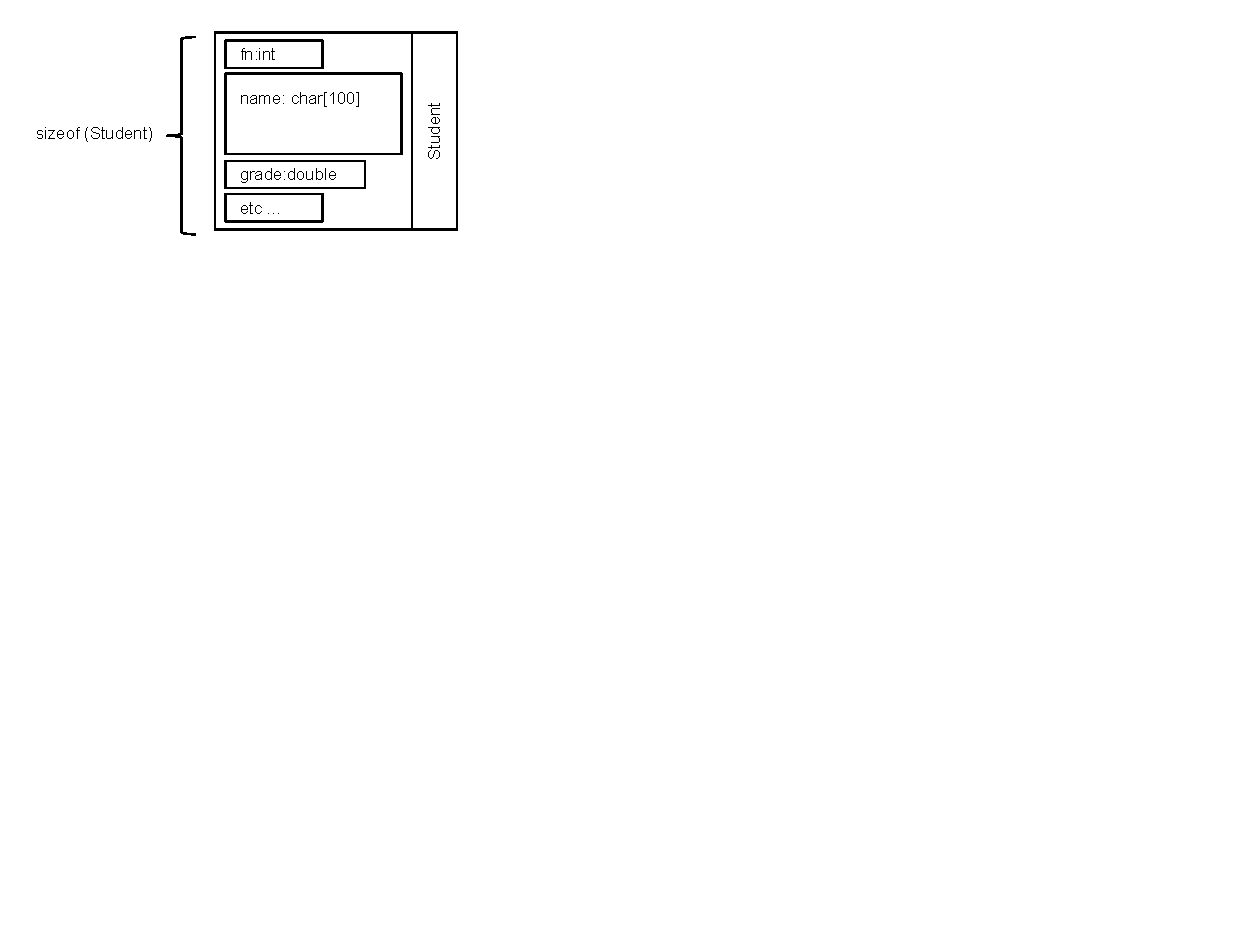
\includegraphics[width=16cm]{images/structstudent}
  \end{column}
\end{columns}


\end{frame}



\begin{frame}[fragile]
\frametitle{Презаписване}

\vspace{-20px}



\begin{columns}[t]
  \begin{column}{0.65\textwidth}

\begin{flushleft}
\relscale{0.70}
\begin{lstlisting}
Student s;
fstream file ("stundets.bin", 
              ios::in | ios::out | 
              ios::binary);

file.seekg(2*sizeof(Student));
file.read ((char*)&s, sizeof (Student));

s.deleted = true; //!!!

file.seekp(2*sizeof(Student));
file.write ((char*)&s,sizeof (Student));
\end{lstlisting}
\end{flushleft}   


  \end{column}
  \begin{column}{0.35\textwidth}
\begin{flushright}
\relscale{0.65}
  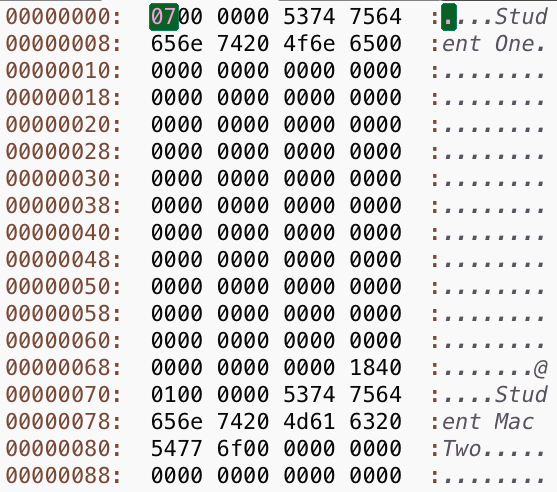
\includegraphics[width=4.0cm]{images/binfiless}
\end{flushright}

  \end{column}
\end{columns}

\vspace{10px}
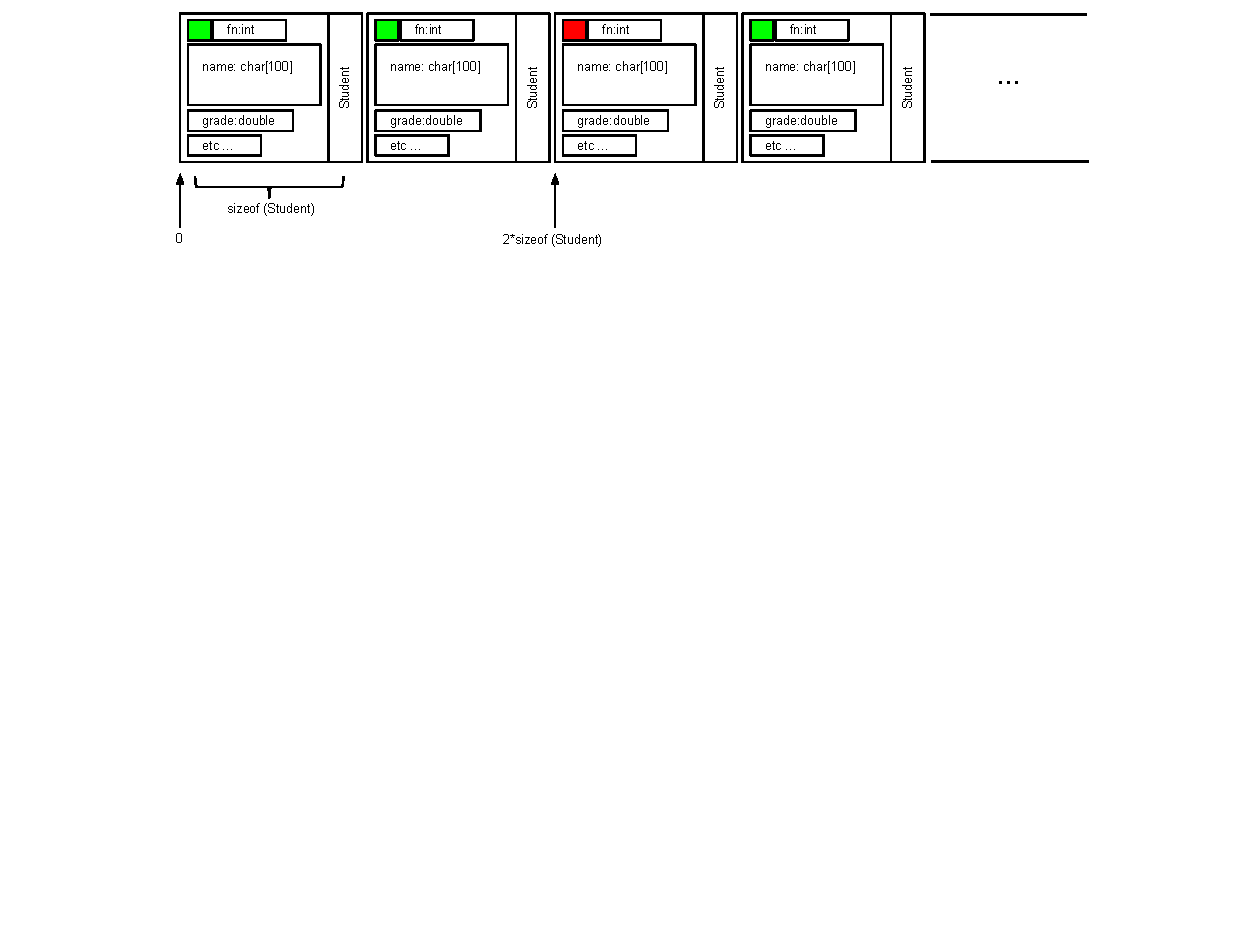
\includegraphics[width=12cm]{images/binfileflag}


\end{frame}

\begin{frame}[fragile]
\frametitle{Добавяне на ``свободно'' място или в края}

\vspace{-20px}



\begin{columns}[t]
  \begin{column}{0.65\textwidth}

\begin{flushleft}
\relscale{0.65}
\begin{lstlisting}
Student s,tmp;//...
fstream file ("stundets.bin", 
              ios::in | ios::out | 
              ios::binary);

file.seekg(0);
while (file.read ((char*)&tmp, 
                  sizeof (Student)) &&
       tmp.deleted == false){};

if (tmp.deleted == true)
  file.seekp (file.tellg()-sizeof(Student));

file.write ((char*)&s,sizeof (Student));
\end{lstlisting}
\end{flushleft}   


  \end{column}
  \begin{column}{0.35\textwidth}
\begin{flushright}
\relscale{0.65}
  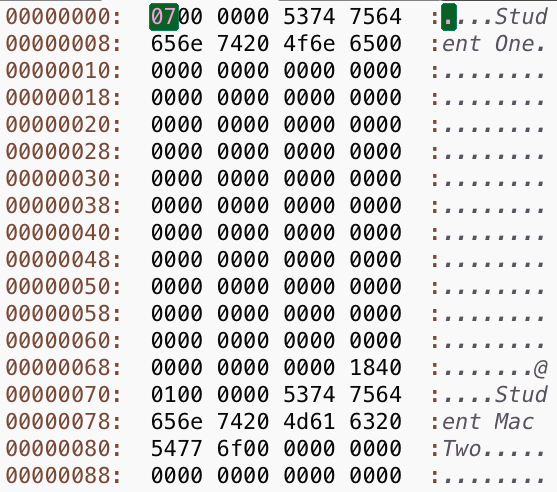
\includegraphics[width=4.0cm]{images/binfiless}
\end{flushright}

  \end{column}
\end{columns}

%\vspace{4px}
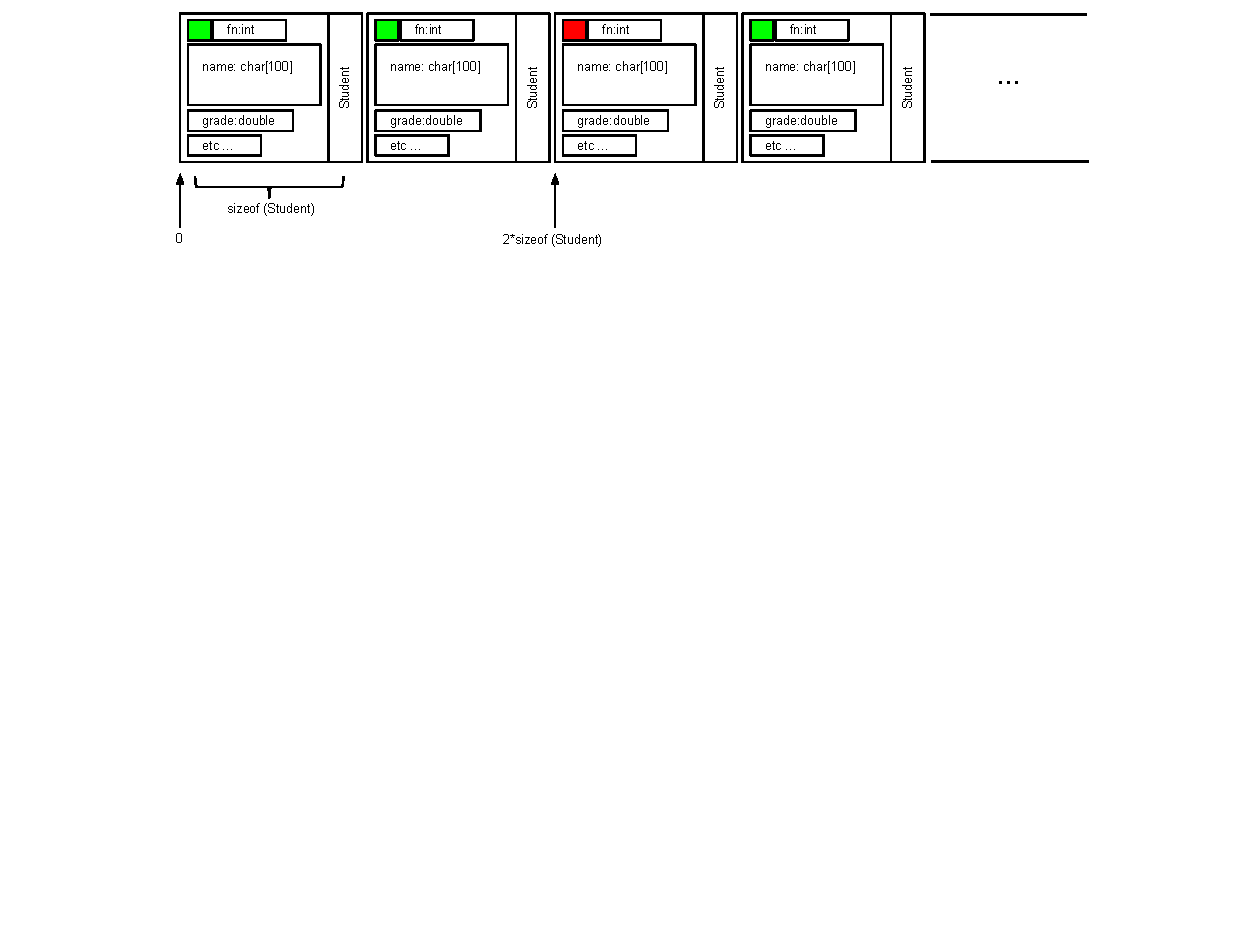
\includegraphics[width=12cm]{images/binfileflag}


\end{frame}



\begin{frame}[fragile]
\frametitle{Подравняване}

\vspace{-20px}



\begin{columns}[t]
  \begin{column}{0.6\textwidth}

\begin{flushleft}
\relscale{0.70}
\begin{lstlisting}
    struct Student
      {
        int fn;
        char name[100];
        double grade;
        //others
      };
\end{lstlisting}
\end{flushleft}   

  \end{column}
  \begin{column}{0.4\textwidth}
\begin{flushright}
\relscale{0.65}
  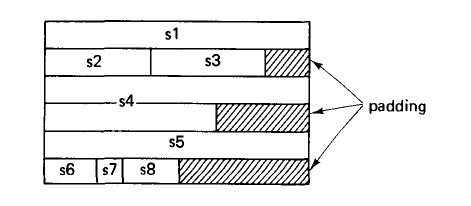
\includegraphics[width=5.0cm]{images/padding}
\end{flushright}

  \end{column}
\end{columns}

\begin{remark}[]
    $sizeof(Student) \ge sizeof (int)+100*sizeof(char)+sizeof(double)$
\end{remark}      


\begin{columns}[t]
  \begin{column}{0.5\textwidth}

\begin{flushleft}
\relscale{0.70}
\begin{lstlisting}
  file.read ((char*)&s.fn,
             sizeof(int));
  file.read ((char*)&s.name,
             100*sizeof(char));
  file.read ((char*)&s.grade,
             sizeof(double));
\end{lstlisting}
\end{flushleft}   

  \end{column}
  \begin{column}{0.5\textwidth}


\begin{flushleft}
\relscale{0.70}
\begin{lstlisting}
  file.read ((char*)&s,
             sizeof(Student));
\end{lstlisting}
\end{flushleft}   

  \end{column}
\end{columns}

\end{frame}


\begin{frame}
\centerline{Благодаря за вниманието!}
\end{frame}

\end{document}




\begin{columns}[t]
  \begin{column}{0.2\textwidth}

  \end{column}
  \begin{column}{0.8\textwidth}

  \end{column}
\end{columns}
